\section{Hardware}
Drahtlose Ad-hoc oder Sensornetzwerke erm"oglichen 
die Verbindung von Netzwerken zwischen zwei oder mehreren Endger"aten. 
Die Ger"ate verbinden sich ohne feste Infrastruktur. Dies f"uhrt dazu, 
dass f"ur die Kommunikation keine festen Routingknoten 
bestehend aus Datenspeicher, Sensoren, Stromquelle und 
Funkmodul ben"otigt werden. Dar"uber hinaus haben sie mehrere 
Optionen f"ur den Aufbau eines Sensorknotens und die Entwicklung, 
um von mehreren Anwendungen zu profitieren.    
Zu Beginn der 70er Jahre wurden die ersten AD-Hoc-Netze vom US-Milit"ar 
entwickelt und werden heute noch im zivilen Bereich verwendet. 
Um einen drahtlosen Sensor in Arduino zu optimieren, 
m"ussen die Hardwarekomponenten getestet werden. 
Im weiteren Verlauf des Prozesses werden 
einige Versionen von Arduino dargestellt.[18]

\subsection{Die Versionen von Arduino}

Arduino ist eine Open-Source-Elektronikplattform, 
die auf einfach zu bedienender Hard- und Software aufbaut. 
Arduino-Karten sind in der Lage, die Eing"ange -
 das Licht eines Sensors, 
 einen Finger auf einer Taste oder eine Twitter-Mitteilung 
 zu lesen und zu einem Ausgang zu machen,um einen Motor zu schalten, 
 eine LED einzuschalten, 
 etwas online zu ver"offentlichen. 
 Sie k"onnen ihrer Karte mitteilen, was sie tun soll, 
 indem Sie eine Reihe von Befehlen an den Mikrocontroller 
 auf der Karte senden. 
 Dazu wird die Programmiersprache Arduino 
 (basierend auf Verkabelung)benutzt und die Arduino-Software (IDE)  
  auf die Verarbeitung basiert[19].
Im Laufe der Jahre war Arduino der Kopf hinter Tausenden von Projekten, 
von Alltagsgegenst"anden bis hin zu komplizierten wi"senschaftlichen
Instrumenten. Eine internationale Gemeinschaft von Studenten, 
Amateuren, K"unstlern, Programmierern und Profis haben sich um diese 
Open-Source-Plattform angesiedelt, ihre Beitr"age haben 
zu einer unglaublichen Menge an zug"anglichem Wissen gef"uhrt, 
das f"ur Anf"angern und Experten eine gro"se Hilfe sein kann.

Arduino wurde am Ivrea Interaction Design Institute als 
leichtes Werkzeug f"ur Rapid Prototypen f"ur Studenten ohne Elektronik
 und Programmierausbildung entwickelt[20]. 
 Als die Arduino-Karte eine breitere "Offentlichkeit erreichte, 
 begann sie sich an neue Anforderungen und Probleme anzupassen 
 und unterscheidet ihr Angebot von einfachen 8-Bit-Karten 
 "uber Produkte f"ur IoT-Anwendungen, Laptops, 3D-Druck und 
 integrierte Umgebungen. Alle Arduino-Karten sind komplett 
 Open Source, so da"s die Benutzer sie selbstst"andig entwickeln 
 und an ihre spezifischen Bed"urfnisse anpassen k"onnen. 
 Die Software ist auch Open Source, 
 und sie wird mit den Beitr"agen von Anwendern 
 auf der ganzen Welt gewachsen..[21]

\subsection{ATmega328 Boards}
\subsubsection{Definition}

Der ATmega328 ist ein von Atmel entwickelter Ein-Chip-Mikrocontroller 
aus der megaAVR-Familie (sp"ater wurde Atmel von Microchip Technology 
im Jahr 2016 "ubernommen). Es verf"ugt "uber einen modifizierten 
8-Bit-RISC-Prozessorkern mit Harvard-Architektur.
Ab 2013 wird der ATmega328 h"aufig in vielen Projekten und autonomen 
Systemen eingesetzt, in denen ein einfacher, 
stromsparender und kosteng"unstiger Mikrocontroller ben"otigt wird. 
Die wahrscheinlich h"aufigste Implementierung dieses Chips ist die 
beliebte Arduino-Entwicklungsplattform, n"amlich die Modelle Arduino 
Uno und Arduino Nano[22].

\subsubsection{Eigenschaften}
Der Atmel 8-Bit-AVR-RISC-basierte Mikrocontroller kombiniert 
32-kB-ISP-Flash-Speicher mit Lese- und Schreibfunktionen, 
1-kB-EEPROM, 2-kB-SRAM, 23 Allzweck-E / A-Leitungen, 32 
Allzweck-Arbeitsregister, drei flexible Timer / Z"ahler mit 
Vergleichsmodi, internen und externen Interrupts, seriell 
programmierbarem USART, einer byteorientierten seriellen 
2-Draht-Schnittstelle, seriellem SPI-Port, 6-Kanal-10-Bit-A / D-Wandler 
(8 Kan"ale in TQFP- und QFN / MLF-Paketen) , programmierbarer Watchdog-Timer mit 
internem Oszillator und f"unf per Software w"ahlbaren Energiesparmodi. 
Das Ger"at arbeitet zwischen 1,8 und 5,5 Volt. Das Ger"at erreicht 
einen Durchsatz von ann"ahernd 1 MIPS pro MHz[23].




\subsection{Arduino Uno}

In der Abbildung~\ref{fig:Uno} ist ein Arduino Uno,der ein Mikrocontroller-Board auf Basis des ATmega328P ist. 
Es besitzt 14 digitale Ein-/Ausgangspins 
(einschlie"slich 6 PWM-Ausg"ange), 6 analoge Eing"ange, 
einen 16 MHz Quarz, einen USB-Anschluss, eine Steckdose, 
einen ICSP-Anschluss und eine Reset-Taste. Es enth"alt alles, 
was man braucht, um den Mikrocontroller zu unterst"utzen; 
der wird einfach "uber ein USB-Kabel an einen Computer 
angeschlossen oder der wird  mit einem AC/DC-Adapter oder einer 
Batterie eingeschaltet, um  ihn zu starten. Man kann an UNO arbeiten, 
ohne  Sorgen zu machen, etwas falsch zu machen, 


 Uno bedeutet eins auf Italienisch und wurde anl"asslich 
 der Ver"offentlichung von Arduino Software (IDE) 1.0 ausgew"ahlt. 
 Die Uno-Karte und die Arduino-Software Version 1.0 (IDE)
 waren die Referenzversionen von Arduino, 
 die sich nun zu neuen Versionen weiterentwickelt haben. 
 Die Uno-Karte ist die erste aus einer Reihe von Arduino USB-Karten 
 und das Referenzmodell f"ur die Arduino-Plattform; eine komplette 
 Liste der derzeitigen, vergangenen und veralteten Karten findet man 
 im Arduino-Kartenverzeichnis [21].
\begin{figure}[!htb]
\begin{center}
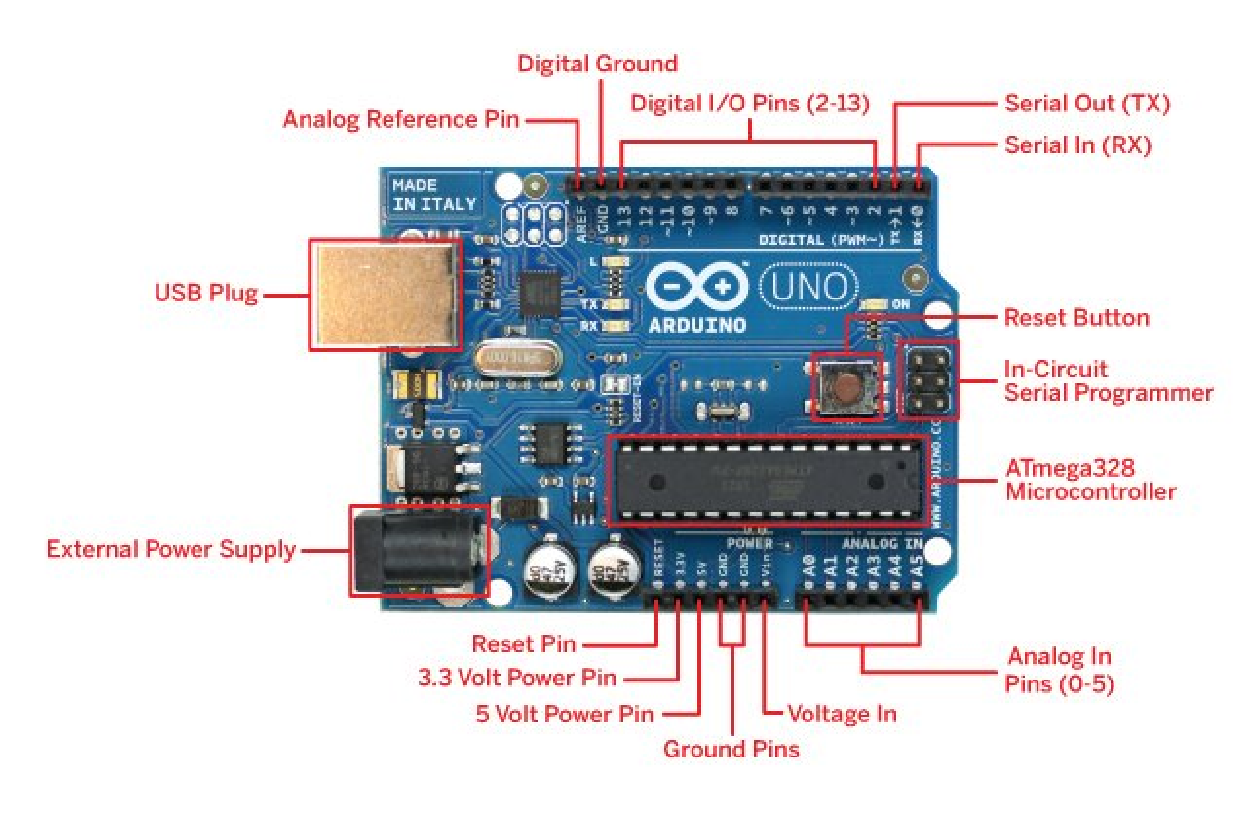
\includegraphics[height=7cm]{bilder/Uno.eps}
\end{center}
\caption{Arduino Uno (eigene Darstellung)}\label{fig:Uno}
\end{figure}



\subsection{ATmega2560}
\subsubsection{Definition}

Das Arduino Mega 2560 ist ein Mikrocontroller-Board, das auf dem 
ATmega2560 basiert. Es verf"ugt "uber 54 digitale Eingangs- / Ausgangspins 
(von denen 14 als PWM-Ausg"ange verwendet werden k"onnen), 16 analoge Eing"ange,
 4 UARTs (serielle Hardware-Ports), einen 16-MHz-Quarzoszillator, 
 einen USB-Anschluss, eine Netzbuchse, einen ICSP-Header und 
 eine Reset-Taste. Es enth"alt alles, was zur Unterst"utzung des 
 Mikrocontrollers ben"otigt wird. Schlie"sen Sie es einfach mit 
 einem USB-Kabel an einen Computer an, oder versorgen Sie es mit 
 einem Netzteil oder Akku, um loszulegen. Das Mega ist kompatibel mit 
 den meisten Schilden, die f"ur den Arduino Duemilanove 
 oder Diecimila entwickelt wurden[24].

\subsubsection{Eigenschaften}
Der RISC AVR-basierte 8-Bit-Microchip-Mikrocontroller 
verbindet 256KB ISP-Flash-Speicher, 8KB SRAM, 4KB EEPROM, 
86 gemeinsame I/O-Leitungen, 32 allgemeine Arbeitsregister, 
Echtzeitz"ahler, 6 flexible Betriebsstundenz"ahler mit Vergleichsmodis, 
PWM, 4 USART, 2 Byte serielle 2-Draht-Schnittstelle, 
16-Bit-A/D-Wandler und JTAG-Schnittstelle f"ur chipbasiertes Debugging. 
Das Ger"at schafft einen Durchsatz von 16 MIPS bei 16 MHz und 
funktioniert zwischen 4,5 und 5,5 Volt.
Durch die Ausf"uhrung leistungsf"ahiger Befehle 
in einem einzigen Taktzyklus erreicht das Ger"at einen 
Durchsatz von etwa 1 MIPS pro MHz, 
der den Stromverbrauch und 
die Verarbeitungsgeschwindigkeit ausgleicht[24].

\subsection{Arduino Mega2560}
Arduino Mega 2560 wie beschrieben in Abbildung~\ref{fig:Mega} ist eine Mikrocontroller-Karte auf 
Basis des ATMega2560 mit 54 
digitalen I/O-Pins (davon 14 als PWM-Ausg"ange nutzbar), 
16 analogen Eing"angen, 4 UARTs (serielle Hardwareschnittstellen), 
einem 16 MHz Quarzoszillator, 
einer USB-Schnittstelle, einem Leistungsstecker, 
einem ICSP-Header und einem Reset-Taster. Es enth"alt alles, 
was man braucht, um den Mikrocontroller zu unterst"utzen. 
Man schlie"st die Karte einfach "uber USB an einen Computer an oder man 
schlie"st sie mit einem DC/AC-Adapter oder einer Batterie an, 
um sie zu starten. Arduino Mega ist mit den meisten der 
f"ur Arduino Duo, Duemilanove oder 
Diecimila entwickelten Schilde kompatibel[21].

\begin{figure}[!htb]
\begin{center}
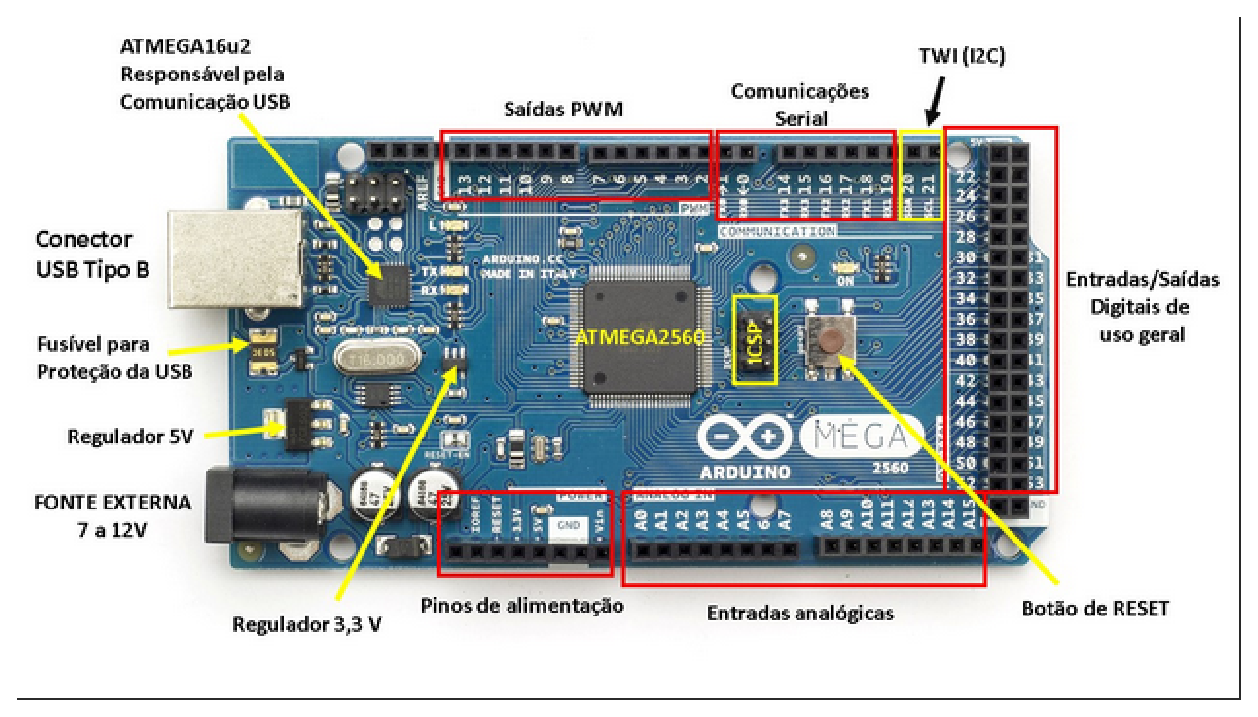
\includegraphics[height=7cm]{bilder/Mega.eps}
\end{center}
\caption{Arduino Mega 2560 Eigene Abbildung in Anlehnung mit[21]}\label{fig:Mega}
\end{figure}














